\documentclass[]{standalone}

%\usepackage{mathptmx}
%\renewcommand{\familydefault}{\rmdefault}
%\usepackage[T1]{fontenc}
%\usepackage[latin9]{inputenc}
\usepackage{siunitx}
\usepackage{array}
\usepackage{amsmath}
\usepackage{ifthen}
\usepackage{pgfplots}
\pgfplotsset{compat=1.14}
\usepackage{titling, graphicx}
\usepackage{tikz}
\usepackage{upgreek}
\usepackage{amsmath,amsthm}
\usepackage{strtikz}
\usepackage{circledsteps}
\usetikzlibrary{shapes,arrows.meta,intersections,graphs,graphs.standard}
\usetikzlibrary{bending, math,fit}
\usetikzlibrary{calc,intersections,through,backgrounds}
\usetikzlibrary{decorations.markings,decorations.pathmorphing, decorations.pathreplacing}
\usetikzlibrary{patterns}



\begin{document}



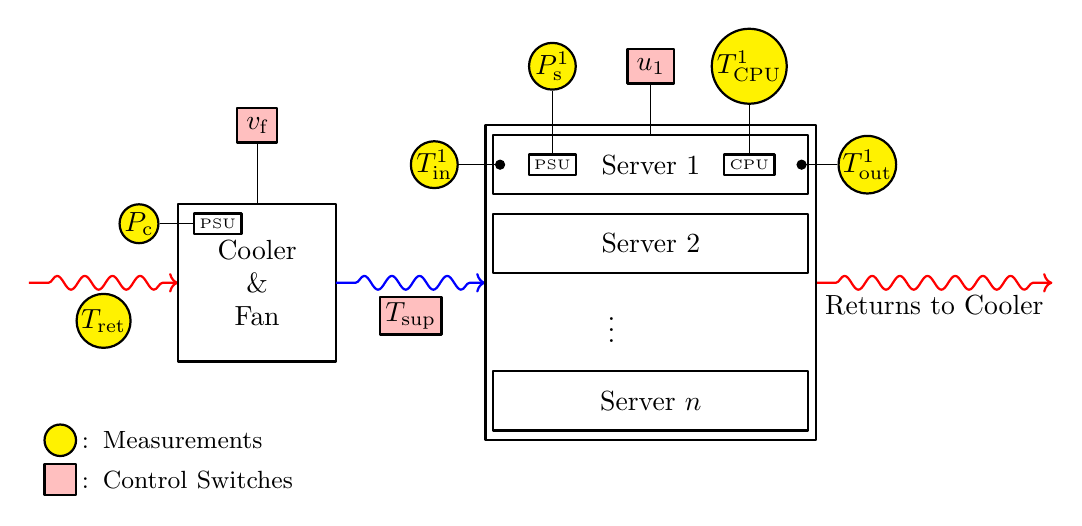
\begin{tikzpicture}[line join=round]
	
\draw[thick, red, ->, decorate,decoration={snake, post length=0.20cm, pre length=0.25cm} ]
(-2.9,0) --  node[black, draw, thick, circle, fill=yellow, below=2pt, inner sep=0.5pt, outer sep=2pt] {$T_\text{ret}$} +(1.9,0);

\node (cooler) at (0, 0) [draw, thick, align=center, minimum width=2cm, minimum height=2cm] {Cooler\\ \& \\Fan};

\node (fanspeed) at (0, 2) [draw, thick, align=center, fill=pink] {$v_\text{f}$};

\draw[] (cooler) -- (fanspeed);

\draw[thick, blue, ->, decorate,decoration={snake, post length=0.20cm, pre length=0.25cm} ]
	(1,0) --  node[black, draw, thick, fill=pink, below=2pt, inner sep=2pt, outer sep=3pt] {$T_\text{sup}$} +(1.9,0);
	
\draw[thick, red, ->, decorate,decoration={snake, post length=0.20cm, pre length=0.25cm} ]
	(7.1,0) --  node[black, below=2pt, inner sep=0.5pt, outer sep=2pt] {Returns to Cooler} +(3.0,0);

\node (server1) at (5, 1.5) [draw, thick, minimum width=4cm, minimum height=0.75cm] {Server $1$};

\node (serverintemp1) at (2.25, 1.5) [draw, thick, align=center, circle, fill=yellow, inner sep=0pt] {$T^1_\text{in}$};
\draw[-{Circle[]}] (serverintemp1) --  ++(0.9,0);

\node (serverouttemp1) at (7.75, 1.5) [draw, thick, align=center, circle, fill=yellow, inner sep=0pt] {$T^1_\text{out}$};
\draw[-{Circle[]}] (serverouttemp1) --  ++(-0.9,0);


\node (cpu1) at (6.25, 1.5) [draw, thick, align=center, minimum width=0.30cm, minimum height=0.20cm, inner sep=2pt] {\tiny{CPU}};
\node (cputemp1) at (6.25, 2.75) [draw, thick, align=center, circle, fill=yellow, inner sep=0.5pt] {$T^1_\text{CPU}$};
\draw[-] (cpu1) -- (cputemp1);

\node (psu1) at (3.75, 1.5) [draw, thick, align=center, minimum width=0.30cm, minimum height=0.20cm, inner sep=2pt] {\tiny{PSU}};
\node (pc1) at (3.75, 2.75) [draw, thick, align=center, circle, fill=yellow, inner sep=0.25pt] {$P_\text{s}^1$};
\draw[] (psu1) -- (pc1);

\node (util1) at (5, 2.75) [draw, thick, align=center, fill=pink] {$u_1$};
\draw[] (server1) -- (util1);

\node (server2) at (5, 0.5) [draw, thick, align=center, minimum width=4cm, minimum height=0.75cm] {Server $2$};
\node (dots) at (4.5, -0.5) [] {\vdots};
\node (servern) at (5, -1.5) [draw, thick, align=center, minimum width=4cm, minimum height=0.75cm] {Server $n$};

\node (servern) at (5, 0.0) [draw, thick, align=center, minimum width=4.2cm, minimum height=4cm] {};


\node (legend0) at (-2.5, -2.0) [draw, thick, circle, fill=yellow, minimum width=0.4cm, minimum height=0.4cm] {};
\node (legend0text) at (-0.85, -2.0) [align=left, text width=2.75cm] {\small: Measurements};

\node (legend0) at (-2.50, -2.5) [draw, thick, fill=pink, minimum width=0.4cm, minimum height=0.4cm] {};
\node (legend0text) at (-0.75, -2.5) [align=left, text width=2.95cm] {\small: Control Switches};

\node (psucool) at (-0.5, 0.75) [draw, thick, align=center, minimum width=0.30cm, minimum height=0.20cm, inner sep=2pt] {\tiny{PSU}};
\node (pccool) at (-1.5, 0.75) [draw, thick, align=center, circle, fill=yellow, inner sep=0.25pt] {$P_\text{c}$};
\draw[] (psucool) -- (pccool);

\end{tikzpicture}




\end{document}
